\chapter{Generazione dei video fake}

\section{Funzionamento}
\label{sec:funzionamento}

\section{Valutazione delle soluzioni disponibili}

Per la generazione dei video fake sono stati valutati tre applicativi diversi, forniti come Software-as-a-Service (SaaS):
\begin{itemize}
    \item DupDub.com
    \item Synthesia.io
    \item HeyGen.com
\end{itemize}

I criteri che sono stati valutati sono: la naturalezza dei movimenti generati, l'estensione dei movimenti generati, la possibilità di generare avatar personalizzati, la qualità del lip-sync\footnote{sincronizzazione tra il movimento delle labbra di un soggetto e il suono delle parole pronunciate.}, la qualità e la naturalezza della voce parlata generata, e il grado di realismo generale dei video generati. Vediamo per ordine i punti di forza e di debolezza identificati di ognuno, e come si è pervenuti alla scelta finale. 

\subsection{DupDub}

DupDub si classifica come un prodotto "Talking-Photo". A partire da una fotografia di un persona, genera il movimento dei muscoli facciali e delle labbra per simulare il parlato. DupDub trova i suoi punti di forza nell'essere molto semplice, ma è stato valutato come troppo semplice per gli scopi di questa ricerca. La più grande limitazione è data dalla limitatezza dei movimenti, limitandosi appunto a generare solo i movimenti dei muscoli facciali, e a malapena movimenti della testa, rendendo il risultato finale poco convincente e innaturale. Permette facilmente la creazione di un avatar personalizzato, a partire da un soggetto noto, ma i movimenti sono stati valutati come molto limitati e innaturali, risultando non idoneo per questa ricerca.

\subsection{Synthesia.io}

Rispetto al precedente, Synthesia.io fornisce avatar in mezzo busto, ed è in grado di generare movimenti del viso, della testa, e anche del corpo, producendo risultati più naturali di DupDub. Gli avatar forniti sono stati generati a partire da persone reali, ed il servizio offre la possibilità di generare dei propri avatar personalizzati. I punti di debolezza individuati sono stati: la qualità del lip-sync e la qualità delle voci generate. In particolare, è risultato frequente il disallineamento tra il movimento delle labbra dell'avatar e il suono della voce generato. La voce inoltre è stata valutata come poco espressiva e poco naturale.

Nonostante questo, tale servizio poteva essere un buon candidato per la ricerca, ma è stato scartato a causa del piano offerto, in quanto offriva un servizio ad abbonamento basato su minuti di video generati.

\subsection{HeyGen}

Sin dal primo sguardo, HeyGen.com si è dimostrato essere al di sopra di tutti gli altri. HeyGen si distingue dalle sue controparti supportando video con sfondi reali, e generando movimenti del corpo avanzati come il movimento delle braccia e il gesticolamento delle mani.

Per la generazione dei video, HeyGen offre due soluzioni:
\begin{enumerate}
    \item Generazione con i modelli di avatar e di voce forniti dalla piattaforma
    \item Creazione di un avatar personalizzato, che a partire da un video di riferimento clona l'aspetto e la voce della persona raffigurata, mantenendo lo sfondo raffigurato
\end{enumerate}

Selezionato il metodo di generazione, si inserisce un testo di riferimento, a partire dal quale verrà generato il video fake.

\subsubsection{Generazione con i modelli di avatar e di voce forniti dalla piattaforma}

La piattaforma fornisce un catalogo di avatar e di modelli di voce già pronti per l'utilizzo. Con questi è possibile generare un video fake utilizzando soltanto un testo di riferimento. È il metodo più veloce per la generazione di video fake, poiché non ha bisogno di un video di riferimento per la creazione di un avatar ad-hoc, e permette di iniziare a generare video immediatamente. Si è, d'altra parte, limitati dall'aspetto degli avatar forniti dalla piattaforma. Gli avatar forniti sono privi di sfondo, per cui il video generato presenta l'avatar al centro dell'inquadratura, posto su uno sfondo bianco. Per la generazione è necessario identificare l'avatar che si intende utilizzare, ed identificare il modello di voce più adatto all'avatar scelto, tra quelli forniti dalla piattaforma. La piattaforma fornisce modelli di voce compatibili con tutte le lingue del mondo, ma tra tutti i modelli forniti, i modelli in lingua inglese sono i più naturali.

\subsubsection{Generazione con avatar personalizzato}

È possibile creare un avatar personalizzato a partire da un video di riferimento. A partire da tale video, la piattaforma identifica la persona raffigurata nel video, e ne crea un suo avatar. L'avatar creato non è privo di sfondo, bensì è inserito nello stesso sfondo in cui è stato registrato il video originale, aumentando il grado di realismo del video prodotto. Nella creazione di questo avatar è anche clonata la voce del soggetto rappresentato, per cui per la generazione dei video fake verrà utilizzata la voce della persona raffigurata, eliminando il problema di dover scegliere il modello di voce più adatto. Inoltre, la piattaforma si è dimostrata in grado di apprendere bene l'inflessione e l'accento della persona raffigurata, producendo risultati naturali indipendentemente dalla lingua parlata. Con questa soluzione è per cui possibile usare anche video in lingua italiana senza compromettere la qualità del risultato prodotto. C'è solo un dettaglio di cui tener conto, per la creazione di un avatar personalizzato è necessario il consenso esplicito in formato video della persona raffigurata che acconsente verbalmente  l'utilizzo della sua immagine per la creazione di un avatar sulla piattaforma.

\subsection{La scelta}

Per queste ragioni, tra le opzioni valutate, HeyGen è stato valutato come il più adatto, in termini di qualità e naturalezza dei risultati prodotti, ed è stato quindi scelto come soluzione per questa ricerca. Sono state valutate entrambe le opzioni offerte da HeyGen per la generazione dei video fake, i cui approcci vengono approfonditi nella prossima sezione. Un altro fattore che sicuramente ha giocato a suo favore è stato anche il piano offerto, il quale permette di generare infiniti video durante il periodo di abbonamento, posto che questi siano sotto i cinque minuti di durata.

\subsubsection{Profilo dei video fake}
Si delinea così il tipo di video che siamo in grado di generare: video raffiguranti una persona che parla, inquadrata a mezzo busto, privi di movimenti di macchina o cambi di inquadrature, e privi di animazioni o scritte che compaiono a corredo. Il video può essere a sfondo bianco (generazione con avatar forniti dalla piattaforma) o con uno sfondo reale (generazione con avatar personalizzato).

Viste le due possibili soluzioni per la generazione dei video fake, sono state valutate due soluzioni diverse per l'acquisizione dei video reali di riferimento:
\begin{itemize}
    \item Generazione di video fake a partire da video scaricati dal web, facendo utilizzo degli avatar già forniti dalla piattaforma per la generazione dei video fake, così facendo si ottengono soggetti diversi tra video real e fake
    \item Generazione di video fake a partire da video registrati con attori, realizzando avatar personalizzati così da avere lo stesso soggetto tra video real e fake
\end{itemize}

Vediamo ora i dettagli di entrambe le soluzioni, riportando l'approccio seguito, e valutando infine i pro e i contro di ogni soluzione.

\section{Video generati da video scaricati dal web}

\subsection{Criterio di ricerca}
È stata utilizzata per la ricerca dei video la piattaforma YouTube. Il criterio di ricerca usato è stato: cercare i video più simili possibili ai video fake che siamo in grado di generare, così da minimizzare le differenze tra video reali e video fake. Minimizzando le differenze tra video reali e video fake massimizziamo le possibilità che diverse percezioni dei video visualizzati siano dovute solo alla natura (reale o fittizia) dei video visualizzati e non ad altri dettagli come ambientazione, soggetto, etc. Per tali ragioni, sono stati cercati video:
\begin{itemize}
    \item frontali, con un soggetto al centro su sfondo bianco
    \item con nessun movimento di macchina o cambi di inquadrature
    \item autodescrittivi, in altre parole non vengono utilizzate immagini, slide o grafici di supporto che vengono esplicitamente referenziati dallo speaker\footnote{questo perché contenuti esplicitamente referenziati dallo speaker reale non sarebbero presenti nel corrispettivo video fake, creando un'incongruenza e rendendo il video fake inefficace.}
    \item con il minor numero di scritte o immagini che compaiono a corredo, preferibilmente nessuna
    \item con i sottotitoli preferibilmente inseriti a mano dall'autore del video, in modo da poter scaricare il copione associato al video più facilmente, per la generazione del video associato
    \item preferibilmente di durata inferiore ai cinque minuti
\end{itemize}

\subsection{Video trovati}

Durante il periodo di ricerca, sono stati trovati quattro video che soddisfano i criteri stabiliti:
\begin{itemize}
    \item \textit{"How to make a GREAT impression - Presentation Tips"} di Expert Academy \\ (\url{https://youtu.be/lZg6H0WqPVY})
    \item \textit{"How to start a pitch or presentation"} di Dominic Colenso \\(\url{https://youtu.be/P2LwuF7zn9c})
    \item \textit{"How to start a presentation"} di Expert Academy \\(\url{https://youtu.be/LrjlW00kkws})
    \item \textit{"How to Get Over Your Fear of Public Speaking"} di Expert Academy \\ (\url{https://youtu.be/So3Z93hEPDk})
\end{itemize}

I video sono stati scaricati utilizzando il tool open source \verb|yt-dlp| (\url{https://github.com/yt-dlp/yt-dlp}).

\subsection{Processing}

I video individuati non corrispondevano tutti perfettamente alle specifiche richieste, per cui per poterli integrare nella ricerca è stato necessario fare del pre-processing.

\subsubsection{Trimming}

Tutti i video individuati presentavano un introduzione e una coda al video, con musiche, scritte o elementi animati. I video individuati sono per cui stati tagliati, in modo da eliminare gli elementi non utili al nostro studio, e mantenere solamente la parte di video parlata. Per il trimming dei video è stato utilizzato il tool open source gratuito \verb|ffmpeg| (\url{https://www.ffmpeg.org}), così da favorire un'operazione veloce e priva di operazioni di re-econding ove possibile.

\subsubsection{Pulizia dello sfondo}

Alcuni dei video individuati presentavano alcuni elementi grafici a comparsa durante la parte parlata del video, come grafici o piccole scritte. Questo è stato valutato come accettabile visto che tali elementi non venivano referenziati esplicitamente dallo speaker, e comparivano solo in sovrapposizione dello sfondo.\footnote{Ricordiamo che tutti i video individuati presentano uno sfondo bianco uniforme, che non cambia nel tempo.} Questo ha permesso la rimozione di tali elementi aggiuntivi tramite una semplice operazione di video-editing, detta mascheramento.

\paragraph{Mascheramento}

Si identifica un fotogramma dell'immagine dove non vi sono elementi a coprire la parte dello sfondo interessata, e si salva tale fotogramma come file a parte. Questo fotogramma "pulito" è detto \textit{clean plate}. Dal momento che lo sfondo è statico, ovvero non cambia nel tempo, il clean plate funge da copia pulita dell'immagine, che possiamo utilizzare per coprire qualunque elemento in sovrapposizione dello sfondo. Con un qualunque programma di editing, si sovrappone il clean plate alla porzione temporale di video in cui compare l'elemento da rimuovere, ad esempio una scritta, e si effettua poi una maschera, che va a ritagliare il clean plate. Come una toppa, il clean plate mascherato copre il testo in sovra-impressione, rimuovendolo dal video. È possibile vedere un esempio di questa operazione in Figura \ref{fig:masking}.

\begin{figure}[ht]
    \centering
    \begin{subfigure}{0.32\textwidth}
        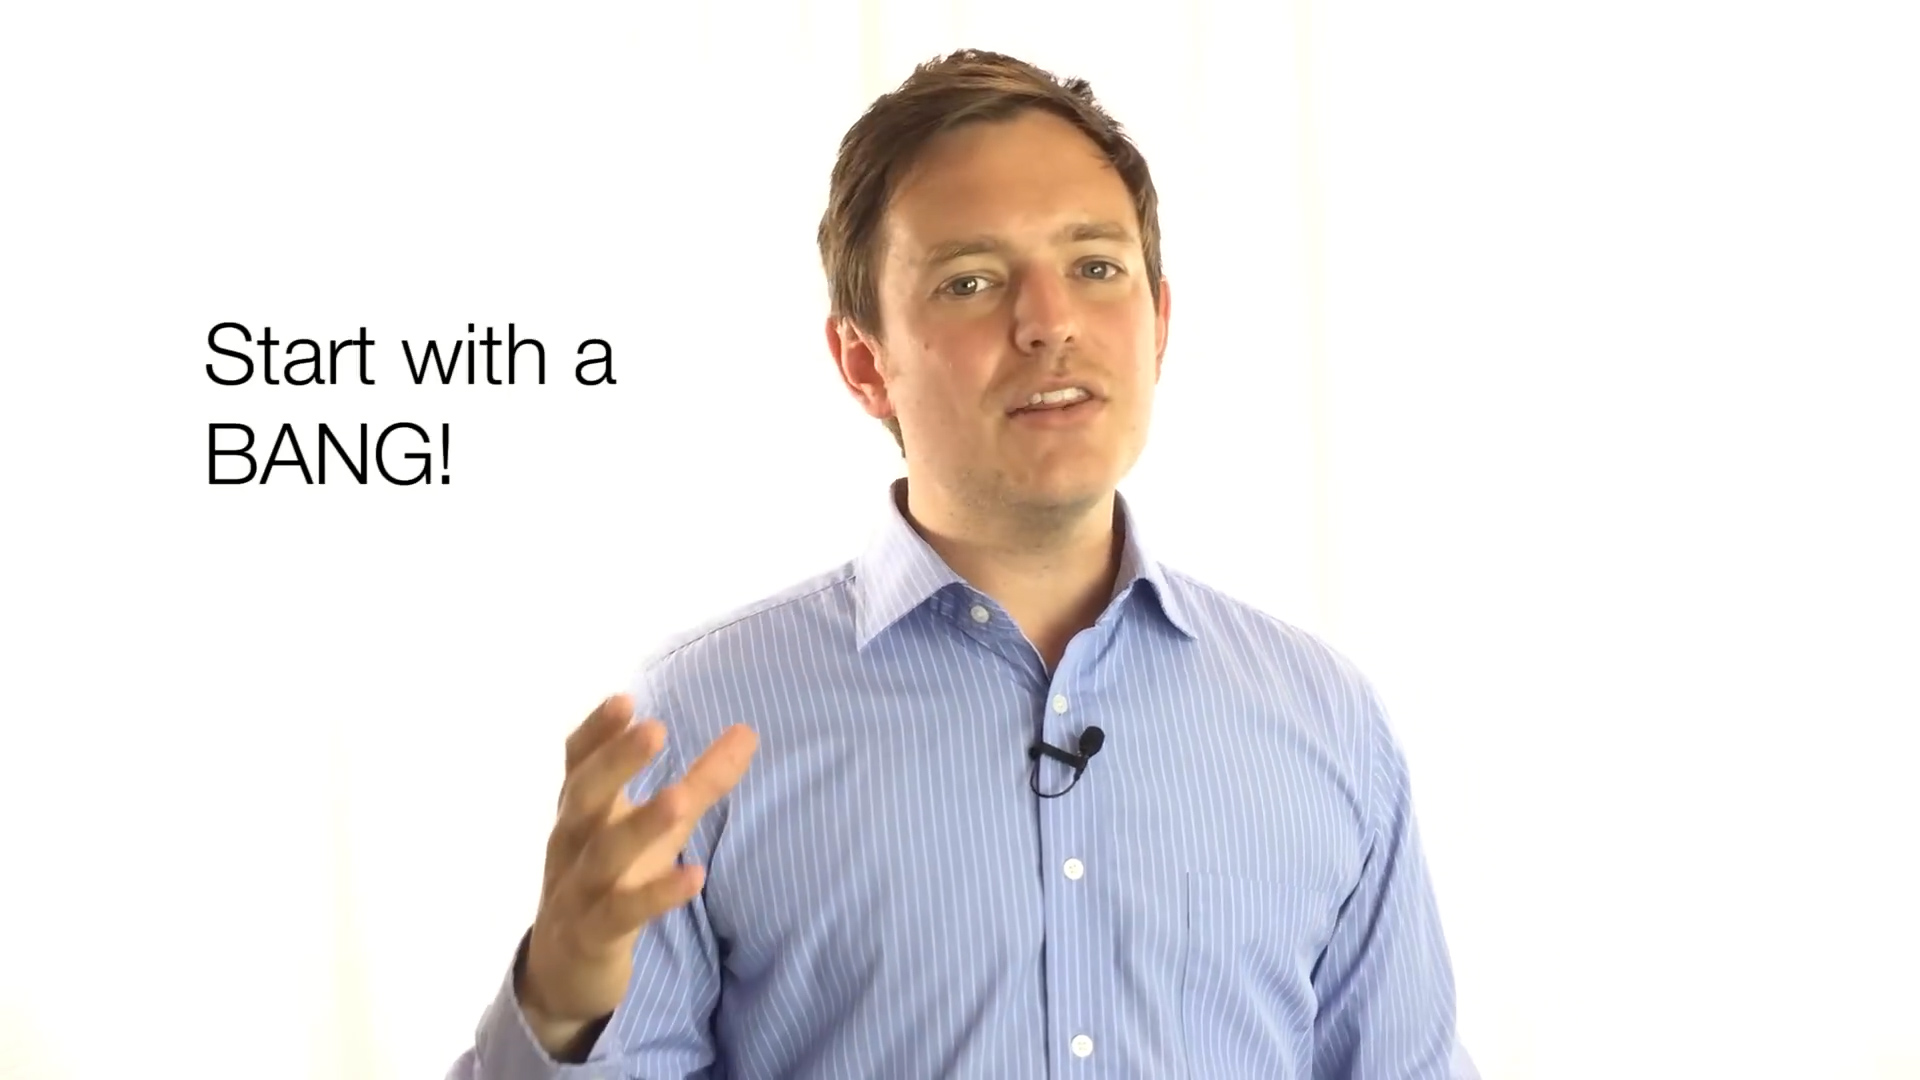
\includegraphics[width=0.95\linewidth]{images/original_frame} 
        \caption{Fotogramma originale}
        \label{fig:original_frame}
    \end{subfigure}
    \hfill
    \begin{subfigure}{0.32\textwidth}
        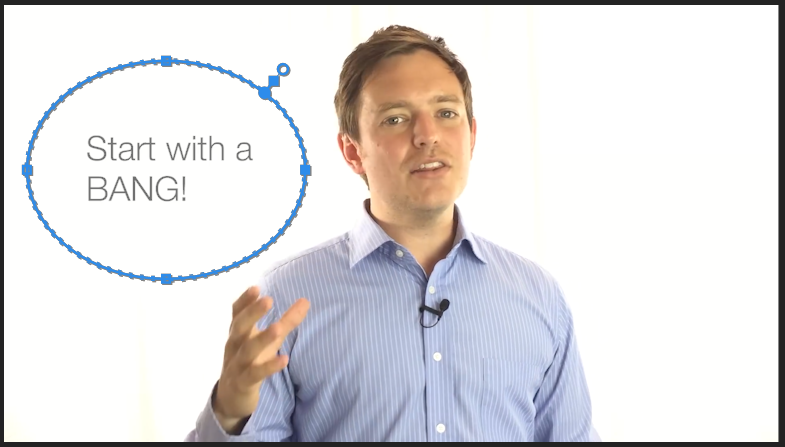
\includegraphics[width=0.95\linewidth]{images/mask_with_text}
        \caption{Maschera sovrapposta}
        \label{fig:mask_with_text}
    \end{subfigure}
    \hfill
    \begin{subfigure}{0.32\textwidth}
        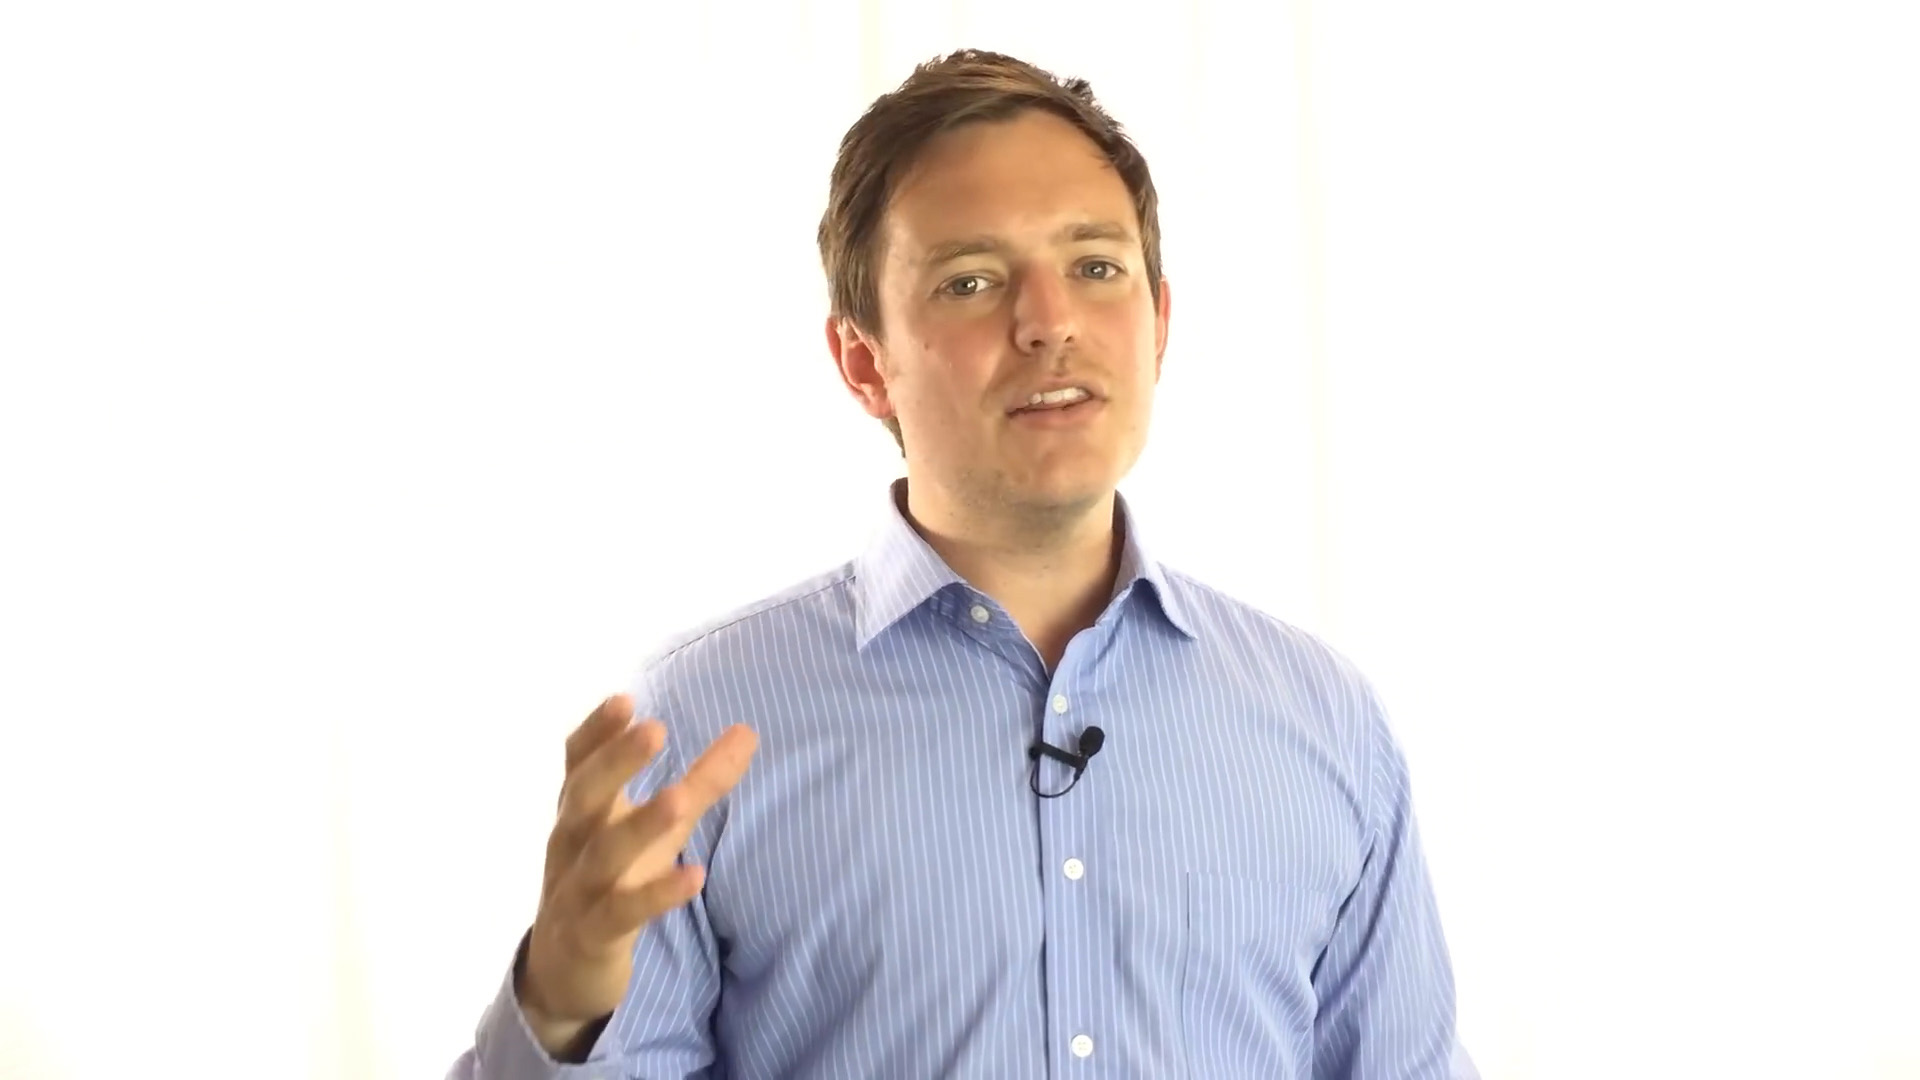
\includegraphics[width=0.95\linewidth]{images/masked}
        \caption{Fotogramma mascherato}
        \label{fig:masked}
    \end{subfigure}
    
    \caption{Una operazione di mascheramento con clean plate in Adobe Premiere Pro}
    \label{fig:masking}
\end{figure}

\subsubsection{Estrazione del testo}
\label{sec:text_extraction}

Per poter generare i doppioni fake, è stato estratto il testo associato al parlato presente nei video individuati. È stato utilizzato il sito web gratuito \url{https://downsub.com} per scaricare i sottotitoli già forniti da YouTube. La maggior parte dei video presentavano dei sottotitoli ufficiali, ovvero inseriti direttamente dagli autori dei video. Per gli altri, sono stati scaricati i sottotitoli generati automaticamente da YouTube, utilizzando quindi di fatto il motore SpeechToText integrato di YouTube.

In ogni caso, tutti i sottotitoli scaricati sono stati poi revisionati a mano per eliminare refusi, errori di battitura o di trascrizione, e per eliminare elementi non parlati o associati alle parti di video che sono state tagliate via. Questi file di sottotitolo sono tutto il necessario per generare i video fake.

\subsection{Generazione dei video fake}

Dal momento che non è possibile ottenere il consenso esplicito dei soggetti rappresentati per la generazione di un avatar personalizzato, è necessario ricorrere agli avatar già forniti dalla piattaforma HeyGen per la generazione dei video fake. Tale processo prevede la selezione di un avatar tra quelli forniti dalla piattaforma, la selezione di una voce tra i modelli TextToSpeech disponibili per generare il parlato, e infine l'inserimento del testo di riferimento.

Per ognuno dei video real individuati sono stati generati due video fake, uno con un avatar di genere maschile e uno con un avatar di genere femminile. Per la generazione di un video fake è stata seguita la seguente procedura, per ogni video real:

\begin{enumerate}
    \item Scelta di un avatar
    \item Scelta del modello di voce più adatto all'avatar scelto
    \item Se non è stata trovata una coppia avatar-voce convincente tornare al passo 1 passando al prossimo avatar
    \item Inserimento del testo estratto dal video real
    \item Fine-tuning del testo per migliorare intonazione, pronuncia e pause
    \item Revisione del risultato, ripetere il passo 5 se necessario
    \item Ripetizione del processo con un avatar del genere opposto
\end{enumerate}

% La procedura di generazione dei video fake ha previsto: la selezione degli avatar da utilizzare tra quelli forniti dalla piattaforma, la scelta della voce da utilizzare, ed eventuali modifiche del testo per migliorare la pronuncia o l'intonazione.

\subsection{Scelta degli avatar}

\begin{figure}[t]
    \centering
    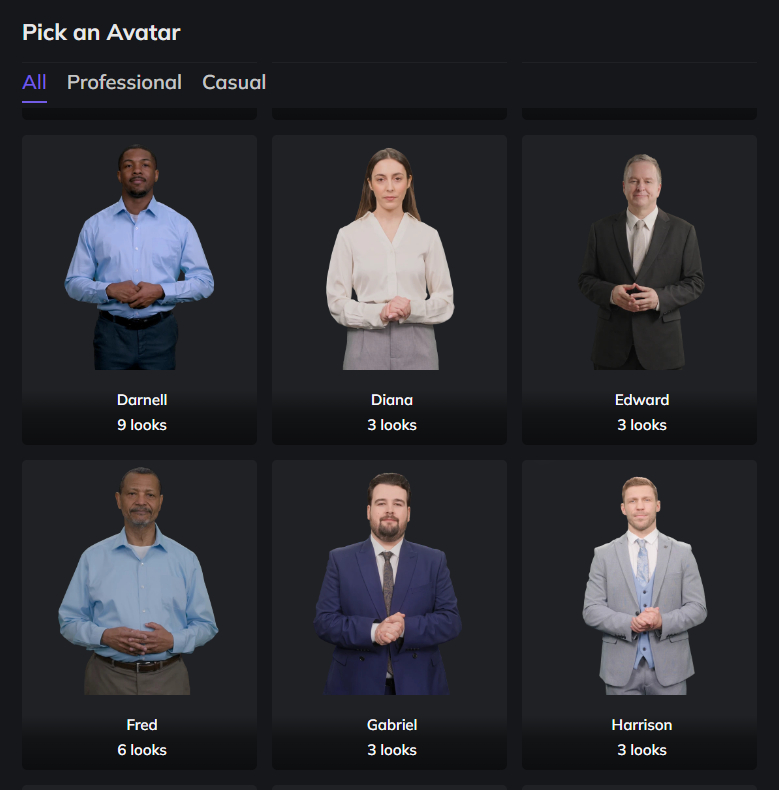
\includegraphics[width=0.62\linewidth]{images/pick_avatar}
    \caption{Esempio di schermata di selezione\\ dell'avatar della piattaforma HeyGen}
    \label{fig:pick_avatar}
\end{figure}

% \begin{figure}[t]
%     \centering
%     \includegraphics[width=0.9\linewidth]{images/heygen_platform}
%     \caption{La piattaforma di generazione HeyGen}
%     \label{fig:heygen}
% \end{figure}

Il punto di partenza per la generazione di un video fake è la scelta dell'avatar da utilizzare, ovvero la persona che verrà animata per realizzare il video parlato. La piattaforma HeyGen mette a disposizione una sua selezione di avatar proprietari, disponibili a tutti gli utenti del servizio, per realizzare i video fake. Gli avatar sono figure di persone a mezzo busto o in primo piano, prive di sfondo. È possibile vedere in Figura \ref{fig:pick_avatar} un esempio ridotto della schermata di selezione degli avatar forniti da HeyGen. Tra gli avatar sono disponibili look molto variegati, tra cui figure in abiti formali, completi, in camice, abiti da lavoro, abiti casual, etc. Per il nostro studio, sono stati considerati avatar con un look semi-formale o casual.

La piattaforma offre anche la possibilità di realizzare un proprio avatar, a propria immagine e somiglianza, ma non è stato possibile nel nostro studio usufruire di questa feature, avendo utilizzato come video real video di terzi.\footnote{È richiesto il consenso esplicito del soggetto rappresentato per realizzare un avatar a sua immagine.} 

% future works: ripetere l'esperimento realizzando video in casa, così da poter avere la stessa persona tra video real e fake

\subsection{Scelta delle voci}

\begin{figure}[t]
    \centering
    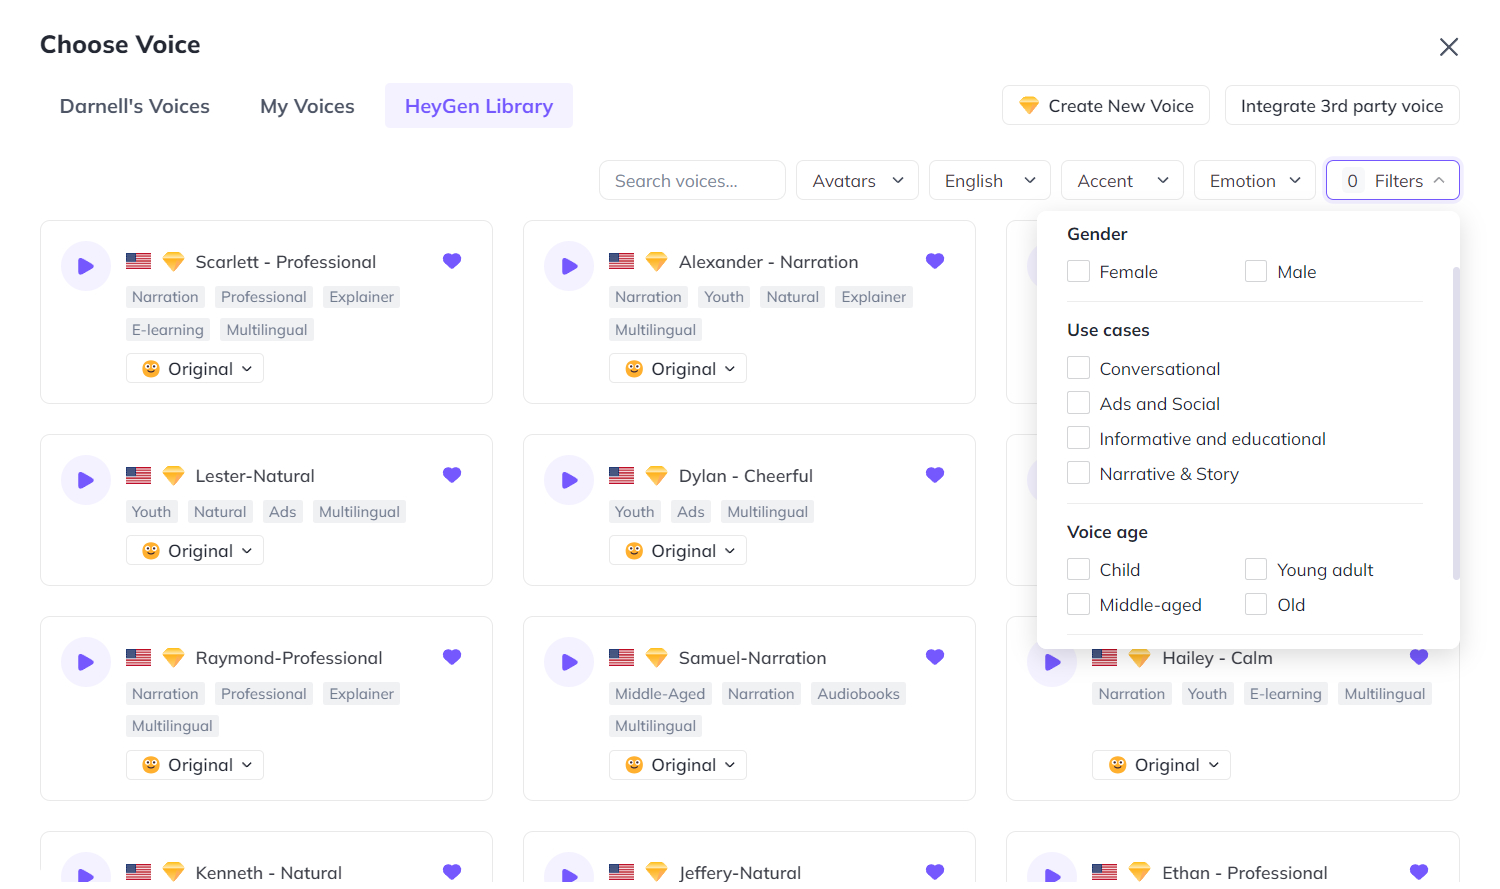
\includegraphics[width=0.9\linewidth]{images/voice_selection}
    \caption{Schermata di selezione della voce sulla piattaforma HeyGen.}
    \label{fig:voice_selection}
\end{figure}

Come anticipato, la scelta degli avatar non è stata fatta in modo indipendente, ma è stata fatta in funzione dei modelli di voce forniti dalla piattaforma HeyGen. Difatti, anche se il video generato è visivamente impeccabile, una voce innaturale o non calzante all'avatar selezionato è in grado di rompere completamente l'illusione, risultando chiaramente artificiale, o può essere un fattore di distrazione, in grado di impedire la fruizione normale del contenuto. Riconosciamo come il giudizio di una proprietà come una voce "calzante al soggetto identificato" può essere fortemente personale, così come anche fortemente umana, e meriterebbe uno studio approfondito a parte. Per i nostri scopi, la scelta è stata guidata dal giudizio umano. 

\subsubsection{Filtraggio tramite categorie di voci}

La piattaforma mette a disposizione un catalogo di voci molto variegato, suddiviso per categorie. Le categorie fornite sono visibili in Figura \ref{fig:voice_selection}, e sono: genere (Maschio, Femmina), età (Child, Young adult, Middle-aged, Old), e "use case" (Conversazionale, Pubblicità e social, Informativo ed educativo, Narrativo). Sono state innanzitutto filtrate le voci selezionando il genere appropriato e la fascia di età appropriata per l'avatar selezionato. In aggiunta, sono state favoreggiate voci categorizzate come a scopo "Informativo ed educativo", ma se necessario sono state valutate anche voci con altri use-case.

\subsubsection{Processo di selezione}

Isolate le possibili voci candidate, è stato generato un video per ogni voce. È stata selezionata poi, tra le candidate, la voce che, visionando il video generato, al giudizio umano è parsa più naturale e convincente con l'avatar selezionato. Se nessuna voce delle voci provate tra quelle fornite dalla piattaforma HeyGen è risultata convincente, l'avatar è stato scartato.\footnote{C'è da notare come con il tempo la piattaforma si è evoluta, e al tempo della scrittura di questo documento, HeyGen fornisce insieme agli avatar una pre-selezione di voci adatte all'avatar selezionato. Questo processo risulterebbe per cui molto semplificato.}

\subsubsection{Lingua} Tutti i video sono stati generati in lingua inglese poiché, sebbene HeyGen fornisca modelli di voci italiane, questi al tempo della ricerca erano limitati in numero e di qualità fortemente limitata rispetto alle controparti anglosassoni.

\subsection{Inserimento del testo}

\begin{figure}[t]
    \centering
    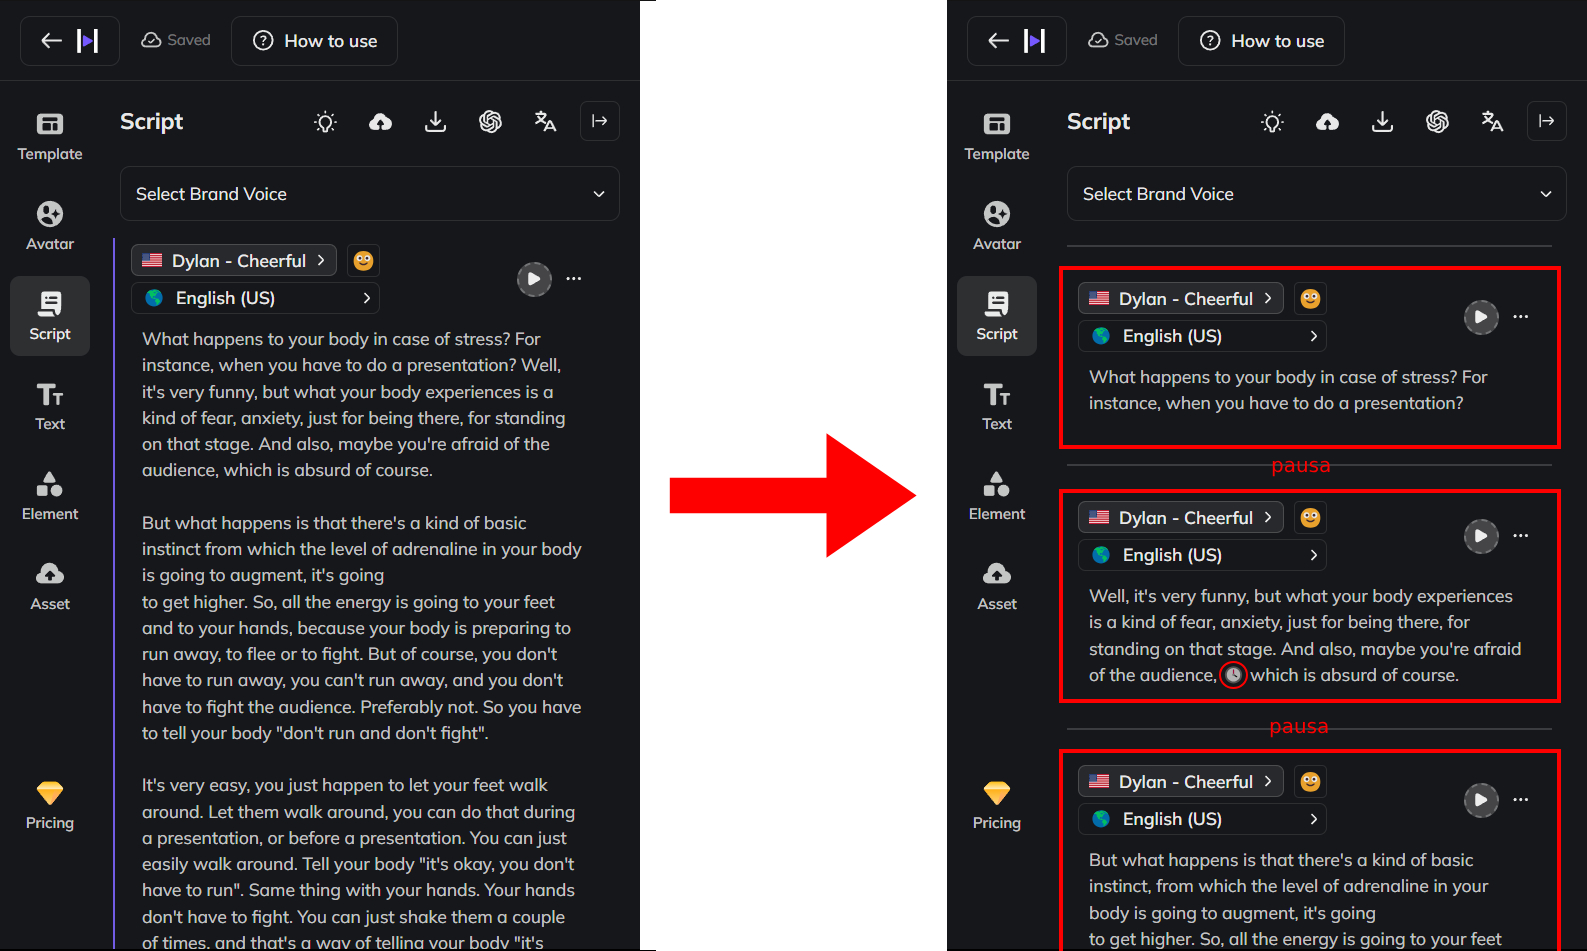
\includegraphics[width=0.9\linewidth]{images/text_heygen}
    \caption{Separazione del testo in paragrafi per introdurre pause naturali.}
    \label{fig:text_heygen}
\end{figure}

L'ultimo passaggio per generare un video fake è l'inserimento del testo da far esporre all'avatar. Nel nostro caso, si tratta del testo estratto dai video real, come spiegato in \ref{sec:text_extraction}. 
I punti chiave di questo passaggio sono: l'introduzione di pause per un flusso naturale del discorso, e la specifica di particolari pronunce, ove necessario.

\subsubsection{Introduzione di pause}
    
La piattaforma HeyGen permette di introdurre pause nel discorso in modo naturale separando il testo in "paragrafi". I paragrafi sono blocchi indipendenti di testo a partire dai quali è generata la voce. Tra un paragrafo e l'altro viene inserita automaticamente una piccola pausa, permettendo un flusso naturale del discorso. È possibile vedere un esempio di separazione in paragrafi in Figura \ref{fig:text_heygen}.

\subsubsection{Revisione del risultato}

A partire dal testo inserito viene generato l'audio della voce, che farà da guida per la generazione dei movimenti dell'avatar, come spiegato in \ref{sec:funzionamento}. Prima di avviare la generazione del video è possibile generare un'anteprima della voce. Se non si identificano problemi di pausa o di pronuncia, si fa partire la generazione del video.

\subsection{Download dei risultati}

Una volta generati i video, questi sono visualizzabili sulla piattaforma e scaricabili gratuitamente in formato 720p o 1080p. I video sono stati scaricati in formato 1080p.

\section{Video generati con attori}

\subsection{Le limitazioni dell'approccio via web}

L'approccio appena presentato è molto semplice e conveniente, in quanto non richiede la registrazione di video appositi per poter realizzare dei video fake, ma presenta delle forti limitazioni. Innanzitutto, il contenuto.

\subsubsection{Complessità del contenuto}

A livello contenutistico, si è limitati dai video che si è in grado di trovare in rete che soddisfano i requisiti richiesti (sfondo bianco, nessun cambio di inquadratura, ecc.). Nonostante la vastità della piattaforma YouTube, i criteri richiesti sono molto specifici, per cui i video trovati sono stati valutati molto limitati, ed in particolare il contenuto, seppur educativo, è stato valutato come di semplice comprensione. Il protocollo sperimentale stabilito prevede la somministrazione di alcune domande di comprensione sui contenuti affrontati, ma se questi sono troppo semplici, la somministrazione di tali domande diventa inefficace nel valutare l'efficacia dell'esperienza. I contenuti esposti nei video devono avere il giusto livello di complessità per essere comprensibili dallo spettatore, ma stimolarne l'attenzione, mettendo alla prova le sue capacità di comprensione.

\subsubsection{Differenza di soggetti tra video reali e video fake}

Un'altra limitazione, più tecnica, è la presenza di soggetti diversi tra un video reale e il video fake associato. Come già detto, individuare i video sul web riduce i tempi di acquisizione dei video, ma ci costringe a usare gli avatar forniti dalla piattaforma HeyGen per la generazione dei video fake. Non è possibile creare degli avatar personalizzati (quindi a immagine e somiglianza) dei video reali, poiché sarebbe necessario il consenso esplicito formato video dei soggetti raffigurati, di cui ovviamente non si può avere a disposizione, essendo i video stati trovati in rete. Bisogna, per cui, utilizzare gli avatar forniti dalla piattaforma HeyGen per realizzare i video. I video reali e i video fake presentano così soggetti diversi.

Seppure entrambi i video sono privi di sfondo, non hanno cambi di inquadratura, immagini o testi di corredo, ecc., non è esattamente vero che l'unica differenza tra i due tipi di video è la loro natura (reale o fittizio). Tra due video che presentano lo stesso argomento con le stesse identiche parole, se i due presentatori sono diversi vi può essere una differenza di percezione nello spettatore, in termini di livello di attenzione, interesse verso l'argomento, e fattore di comprensione degli argomenti esposti. Questo introdurrebbe una variabile esterno che potrebbe influenzare e sporcare i risultati ottenuti, creando differenze tra i dati non dipendenti dal fenomeno che si intende studiare.

\subsubsection{La soluzione}

Entrambi questi problemi trovano una soluzione comune: registrare dei video ad-hoc con attori. Registrando dei video è possibile avere il controllo sul livello di qualità, complessità e sull'argomento trattato nei contenuti esposti, scrivendo un copione preciso da seguire. Inoltre, è possibile fare uso degli avatar personalizzati, garantendo di avere lo stesso soggetto tra video real e video fake, poiché possiamo ottenere il consenso esplicito per la creazione degli avatar di chi si presta come soggetto per il video.

\subsection{Scrittura dei testi}

La realizzazione dei video con attori parte dalla scrittura dei testi che verranno esposti. Come previsto dal protocollo sperimentale, sono stati realizzati due testi, inerenti a due argomenti diversi, di media lunghezza. Questo progetto è stato svolto in collaborazione con l'Università Cattolica del Sacro Cuore, e i testi necessari per la realizzazione dei video sono stati scritti da un tesista dell'Università Cattolica, Matteo Scarinzi, come parte del suo progetto di tesi, seguito dal Prof. Andrea Gaggioli, docente della facoltà di Psicologia della Cattolica.

\subsection{Individuazione degli attori}

Una volta scritti i testi, è stato necessario individuare gli attori disposti a prestare il loro aspetto e la loro voce per registrare i video reali, a partire dai quali vengono realizzati i video fake.

Sono stati cercati un uomo e una donna, di età simile, preferibilmente con già qualche esperienza nell'esporre, spiegare, e parlare in pubblico, per facilitare le operazioni di ripresa dei video. È stato valutato come importante che i due attori avessero età simile per evitare che una chiara differenza di età potesse avere un'influenza diversa sull'esperienza di visione dei video, in termini di comprensione e grado di attenzione e coinvolgimento.

La ricerca è stata effettuata dal tesista della Cattolica Matteo Scarinzi all'interno del corpo docenti e dottorandi della facoltà di Psicologia della Cattolica, seguendo l'intuizione che docenti e dottorandi abbiano buona esperienza nell'esporre argomenti ad alta voce e parlare al pubblico. Sono stati individuati come attori:
\begin{itemize}
    \item Michele Paleologo, per la parte maschile, dottorando della facoltà di Psicologia dell'Università Cattolica del Sacro Cuore
    \item Marta Pizzolante, per la parte femminile, dottoranda della facoltà di Psicologia dell'Università Cattolica del Sacro Cuore
\end{itemize}

\subsection{Acquisizione dei video}

I video sono stati registrati presso la sede dell'Università Cattolica del Sacro Cuore in Via Buonarroti, 30 a Milano, nell'aula privata del Prof. Andrea Gaggioli, docente di Filosofia della Cattolica e collaboratore di questo progetto.

I video sono stati registrati con luce artificiale, così da avere il pieno controllo della luce in scena, e non dipendere dalle condizioni meteo, come il movimento delle nuvole e del sole per la quantità di luce presente in scena durante i video e tra un video e l'altro. Per compensare la luminosità ridotta delle luci della stanza è stata utilizzata una ring light\footnote{Lampada a forma di anello a luce bianca, molto luminosa, che permette attraverso la sua forma caratteristica di illuminare uniformemente il viso senza creare ombre dure sul volto.}, posta davanti la telecamera, così da illuminare gli attori.

Per la acquisizione dei video è di fondamentale importanza che i testi scritti siano seguiti parola per parola dagli attori, per evitare che differenze tra diverse modalità di esposizione possano influenzare i risultati ottenuti. Per garantire ciò senza che gli attori debbano imparare a memoria i testi scritti agli attori, è stato acquistato e utilizzato un teleprompter\footnote{Un meccanismo a specchio che permette, a chi si pone davanti alla telecamera, di leggere il testo senza distogliere lo sguardo dalla camera.}. Per la registrazione dell'audio è stato utilizzato un microfono lavalier wireless. Il setup utilizzato per la registrazione è visibile in Figura \ref{fig:recording_setup}.

Nonostante la capacità del servizio di generazione dei video fake di replicare lo sfondo nei video catturati, i video sono stati registrati di fronte a uno sfondo bianco, per evitare la presenza di possibili elementi di distrazione nello sfondo. È possibile vedere in Figura \ref{fig:recording_session} un esempio della sessione di registrazione.

\begin{figure}[t]
    \centering
    \begin{subfigure}{0.49\textwidth}
        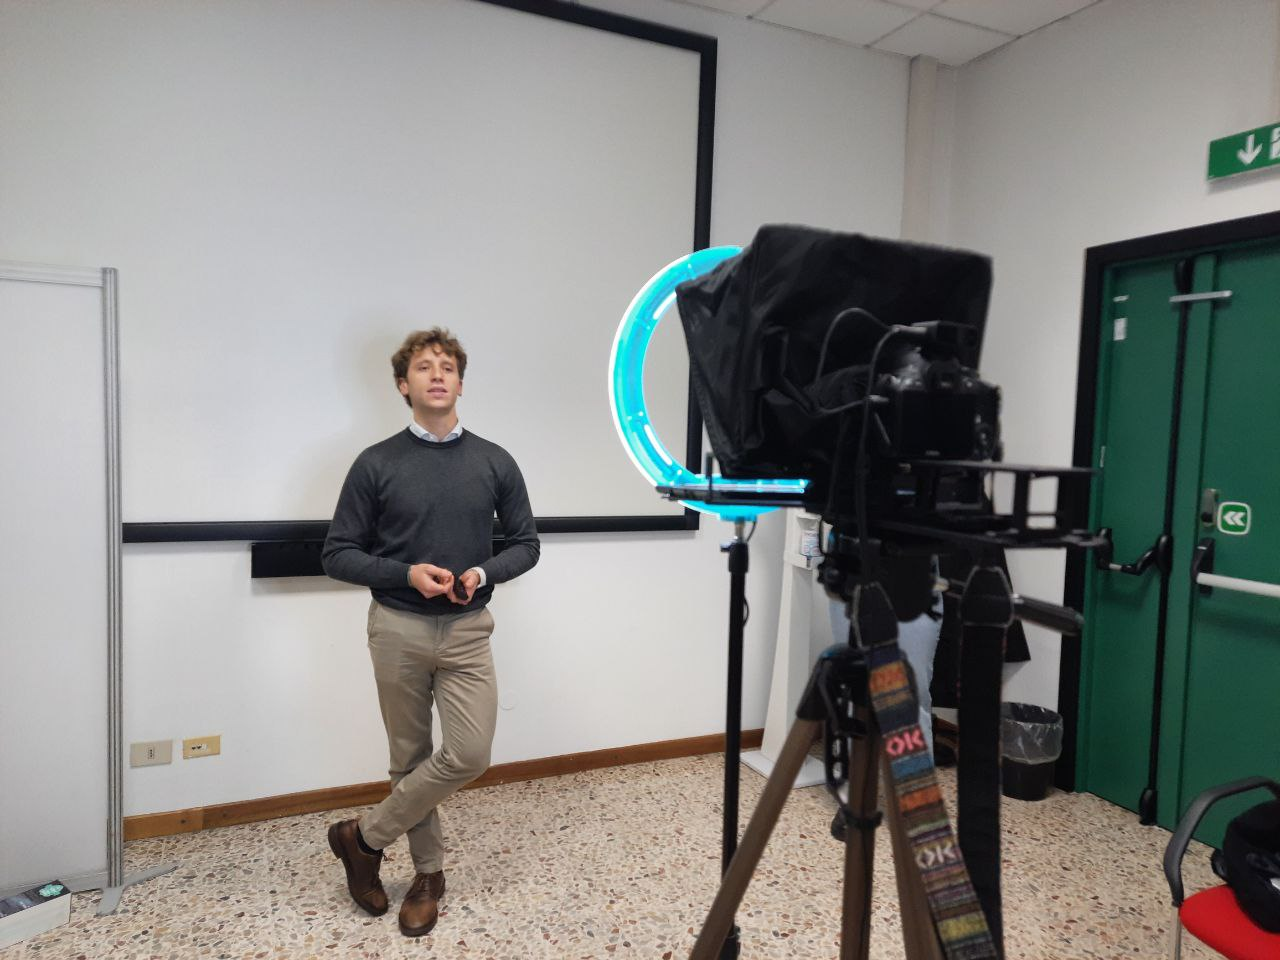
\includegraphics[width=0.95\linewidth]{images/recording_m} 
        \caption{}
        \label{fig:recording_m}
    \end{subfigure}
    \hfill
    \begin{subfigure}{0.49\textwidth}
        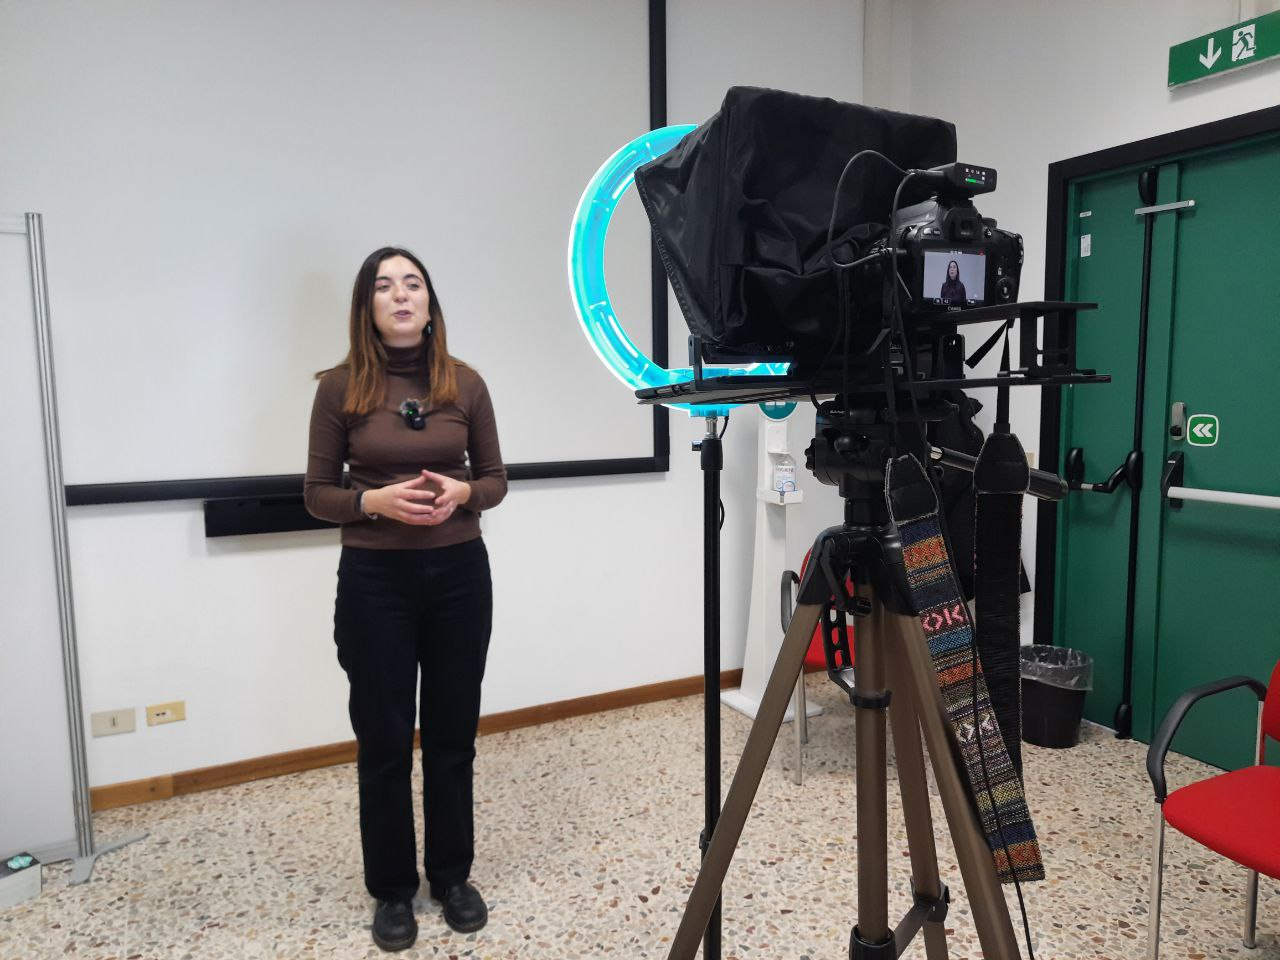
\includegraphics[width=0.95\linewidth]{images/recording_f}
        \caption{}
        \label{fig:recording_f}
    \end{subfigure}
    \hfill
    \caption{Sessioni di registrazione dei video reali con attori, con: (a) Michele Paleologo nella parte maschile, (b) Marta Pizzolante nella parte femminile.}
    \label{fig:recording_session}
\end{figure}

\begin{figure}[t]
    \centering
    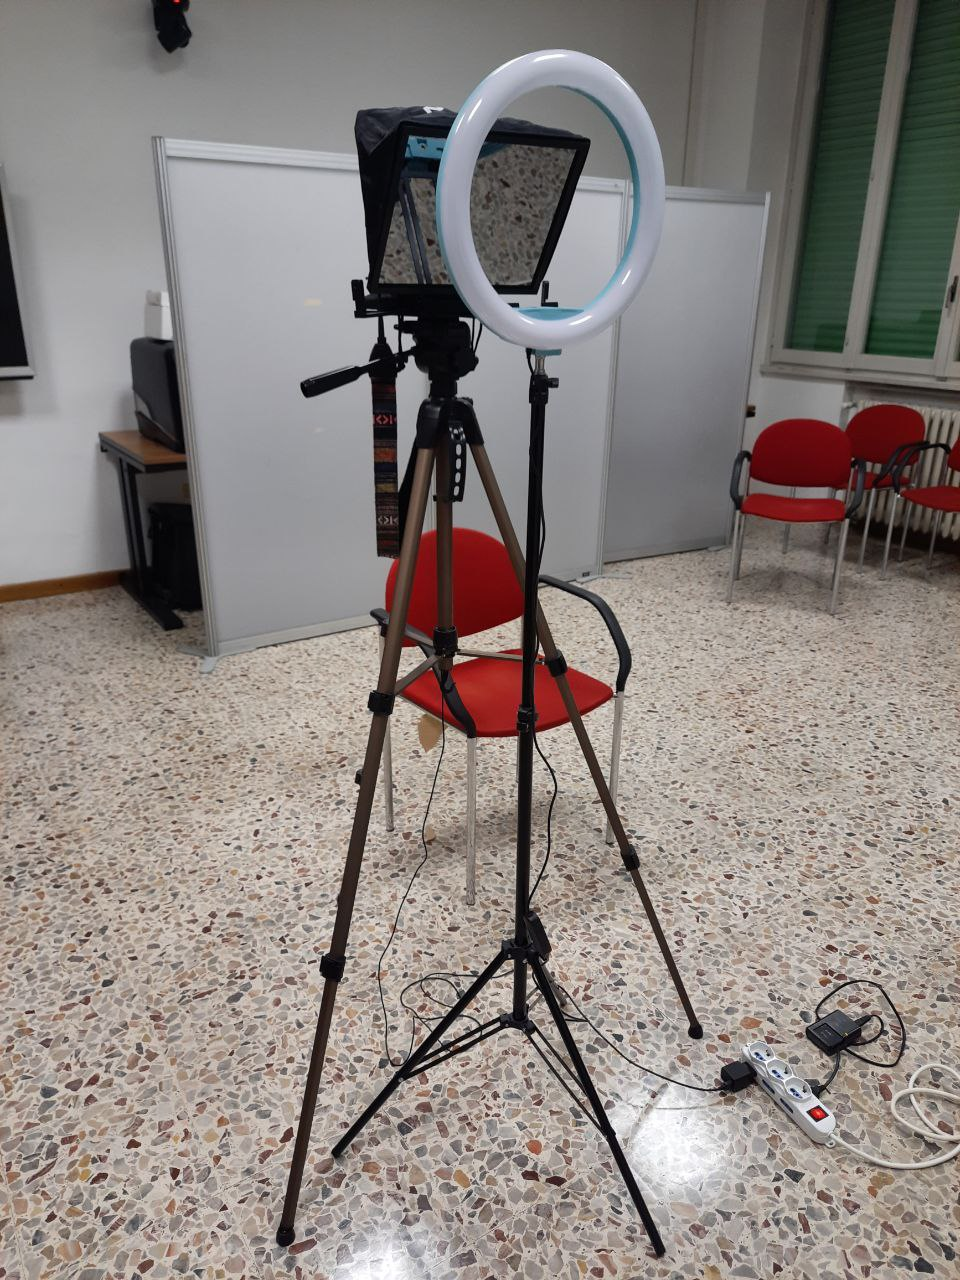
\includegraphics[width=0.4\linewidth]{images/recording_setup}
    \caption{Setup di registrazione dei video fake, con videocamera, teleprompter e ring light.}
    \label{fig:recording_setup}
\end{figure}

\subsubsection{Video di riferimento per la creazione degli avatar}

Per la realizzazione dei video fake è stato registrato per ogni attore un video a parte, richiesto dalla piattaforma HeyGen per la creazione dell'avatar personalizzato (Instant Avatar). La piattaforma richiede un video di breve-media durata, 2-3 minuti, dove si può parlare di qualsiasi argomento. Il video è utilizzato come punto di partenza per creare l'avatar, estraendo da tale video l'aspetto del soggetto, dello sfondo, così come i movimenti del soggetto e il suono della sua voce. Tale video è stato registrato per ogni attore nello stesso identico setup, così che l'avatar realizzato fosse visivamente identico ai corrispettivi video reali. È stato necessario realizzare un video a parte poiché è richiesto dalla piattaforma HeyGen che in tale video vengano inserite frequenti pause tra una frase e l'altra. Questo porta a un flusso del discorso molto innaturale, non rendendo possibile adoperare i video reali per la realizzazione dell'avatar, richiedendo la registrazione di un video dedicato a parte. Tale video è stato processato allo stesso modo di tutti gli altri, così che fosse visivamente e qualitativamente uguale ai corrispettivi video reali.

\subsection{Video processing}

I video registrati sono stati processati per migliorare la qualità dell'immagine. Sono stati applicati un filtro di riduzione del rumore e un aumento della luminosità dell'immagine. Per l'elaborazione dei video è stato utilizzato il programma gratuito Da Vinci Resolve.

\subsubsection{Riduzione del rumore}

\begin{figure}[t]
    \centering
    \begin{subfigure}{0.49\textwidth}
        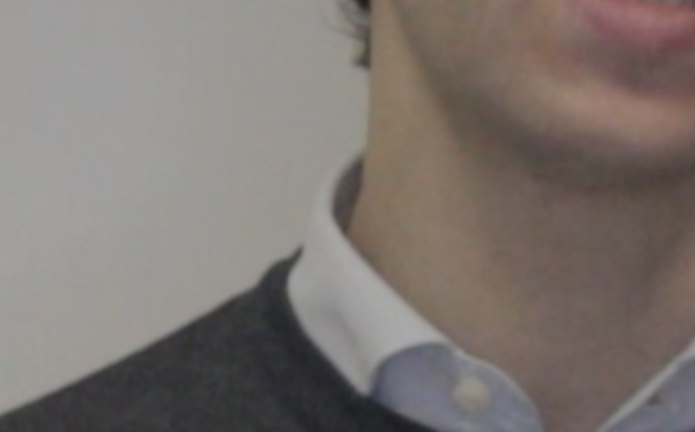
\includegraphics[width=0.95\linewidth]{images/before_nr} 
        \caption{Prima della riduzione del rumore}
        \label{fig:before_nr}
    \end{subfigure}
    \hfill
    \begin{subfigure}{0.49\textwidth}
        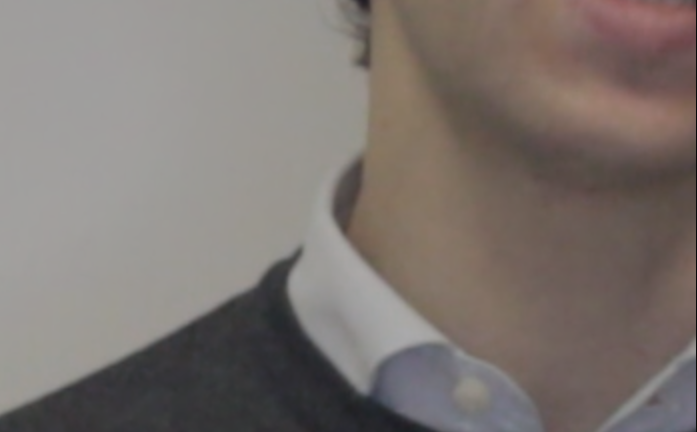
\includegraphics[width=0.95\linewidth]{images/after_nr}
        \caption{Dopo la riduzione del rumore}
        \label{fig:after_nr}
    \end{subfigure}
    \hfill
    \caption{Esempio di filtro di riduzione del rumore dell'immagine nei video con attori.}
    \label{fig:noise_reduction}
\end{figure}

I video sono stati registrati in condizioni di luminosità ristretta, utilizzando la luce artificiale dell'aula a disposizione e una ring light come luce di supporto. Per questo motivo, l'immagine presentava del leggero rumore, che è stato rimosso tramite un filtro di riduzione del rumore, incluso nel programma utilizzato. Il filtro di riduzione del rumore è stato controbilanciato con un filtro di sharpening\footnote{Un aumento della nitidezza dell'immagine, per rendere i dettagli più evidenti.}, per evitare la perdita di dettagli dovuta alla riduzione del rumore. È possibile vedere un esempio del risultato di tale processo in Figura \ref{fig:noise_reduction}\footnote{Si tratta di un esempio molto sottile, e vista la dovuta compressione dell'immagine, necessaria per l'inserimento delle figure in questo documento, e la sua successiva stampa, potrebbe non essere facilmente apprezzabile la differenza tra le due immagini.}.

\subsubsection{Color Grading}

L'immagine è stata migliorata con una correzione del bilanciamento del bianco, per correggere i colori, un leggero aumento della saturazione e della nitidezza, per correggere il profilo neutro della fotocamera utilizzata per le riprese, ed è stata aumentata la luminosità dell'immagine. È possibile vedere un esempio risultato finale in Figura \ref{fig:color_grading}.

\begin{figure}[t]
    \centering
    \begin{subfigure}{0.49\textwidth}
        \includegraphics[width=0.99\linewidth]{images/before_grading} 
        \caption{Immagine originale}
        \label{fig:before_grading}
    \end{subfigure}
    \hfill
    \begin{subfigure}{0.49\textwidth}
        \includegraphics[width=0.99\linewidth]{images/after_grading}
        \caption{Risultato finale}
        \label{fig:after_grading}
    \end{subfigure}
    \hfill
    \caption{Esempio della correzione dell'immagine effettuata su video con attori.}
    \label{fig:color_grading}
\end{figure}

I video sono stati esportati in formato \verb|.mp4|, con codifica H.264 con un target di bitrate di \verb|2048 kb/s|, a \verb|23.976 fps|.

\subsection{Audio Processing}

L'audio registrato è stato normalizzato a un valore di loudness di -23 LUFS (±0.5 LU) integrati (I), secondo lo standard Europeo EBU R128 di distribuzione audio in ambito broadcast. Inoltre, l'audio è stato pulito con un filtro di riduzione del rumore di fondo, ed è stata applicata una curva di equalizzazione (Figura \ref{fig:eq_curve}) e una leggera compressione per rendere l'ascolto più stabile, naturale e gradevole.

L'audio è stato convertito in formato AAC mono a \verb|128 kb/s| per poter essere inserito nel contenitore \verb|.mp4|.

\begin{figure}[t]
    \centering
    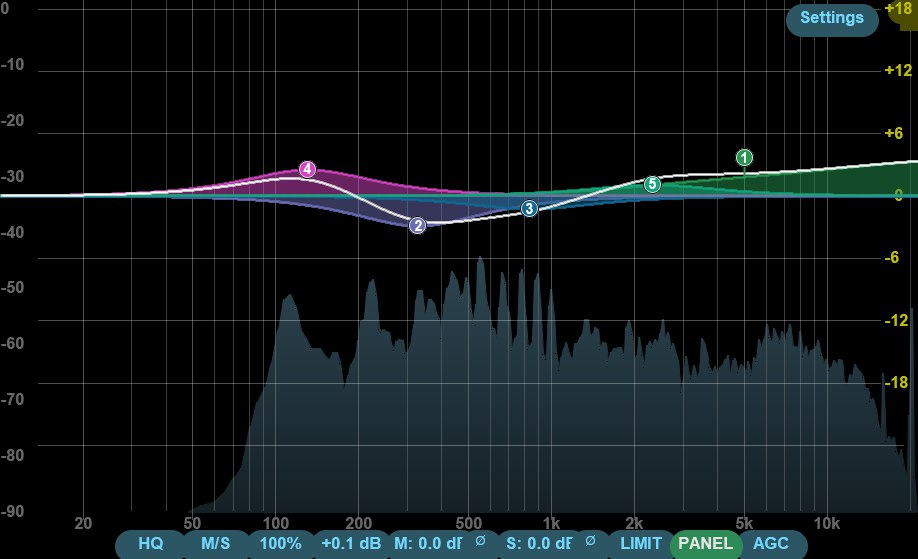
\includegraphics[width=0.62\linewidth]{images/eq_curve}
    \caption{Curva di equalizzazione dell'audio registrato.}
    \label{fig:eq_curve}
\end{figure}

\subsection{Generazione dei video fake}

\clearpage